\section{Outras Implementações}

Neste capítulo, apresentamos versões alternativas do projeto desenvolvido, explorando diferentes abordagens para resolver o problema proposto. Apesar de não termos implementado estas soluções na prática, realizámos simulações utilizando a plataforma \textit{CircuitVerse}, o que nos permitiu observar o seu funcionamento e retirar conclusões relevantes. Estas simulações serviram para avaliar a viabilidade e eficiência das alternativas, oferecendo uma perspetiva mais abrangente sobre possíveis variações do sistema.

\subsection{Implementação com ROM}
Nesta versão, a utilização de uma \gls{rom} foi considerada para armazenar os quadrados de todos os números de 0 a 15. Este método substitui os componentes lógicos tradicionais, permitindo uma abordagem mais compacta e escalável. Por outro lado, introduz limitações relacionadas com o tamanho e a organização da memória.

\begin{figure}[H]
    \centering
    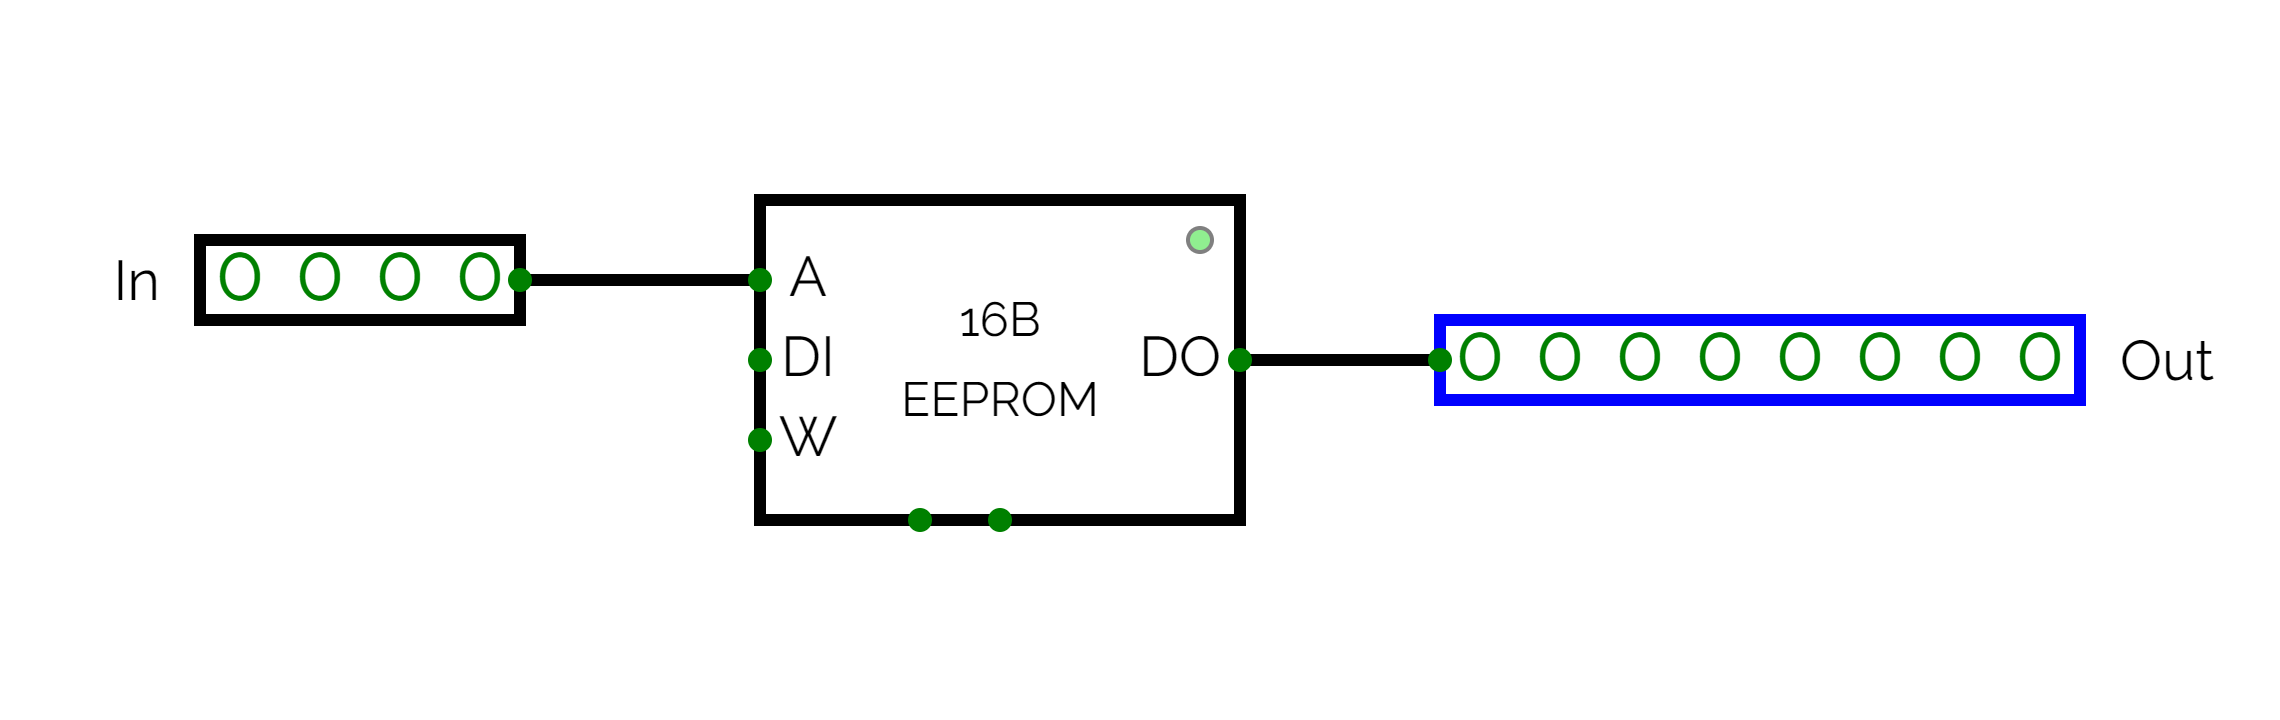
\includegraphics[width=0.8\textwidth]{Implementações/images/ROM.png}
    \caption{Implementação do módulo Quadrado utilizando uma \gls{rom}}\label{fig:QuadradoROM}
\end{figure}

Como é possível observar na figura~\ref{fig:QuadradoROM}, a implementação com uma \gls{rom} reduz significativamente a quantidade de cálculos internos que são realizados. A \gls{rom} é configurada no CircuitVerse através da definição dos valores de saída (representada por DO no módulo da rom) para cada endereço de entrada (representada por A no módulo da rom), correspondendo aos quadrados dos números de 0 a 15. Esta configuração permite que, ao receber um valor de entrada, a \gls{rom} forneça diretamente o resultado pré-calculado, simplificando o circuito e melhorando a eficiência. Por outro lado, a utilização de uma \gls{rom} pode introduzir limitações em termos de escalabilidade e flexibilidade, uma vez que qualquer alteração nos valores armazenados requer a reprogramação da memória.

\subsection{Implementação com contador}
Esta alternativa utiliza um contador para gerar sequências ordenadas de operações e, por um lado, reduz a complexidade do sistema, por outro, aumenta o tempo necessário para efetuar um cálculo. A implementação utiliza um contador binário que decrementa o seu valor a cada ciclo de clock. O contador é controlado pelas entradas D, Load e Enable. A entrada D representa o valor inicial que pretendemos carregar. A entrada Load carrega o valor no contador, e enquanto está ativa bloqueia o seu funcionamento. A entrada Enable, liga e desliga o contador. Quando o Enable é desativado, o contador apaga todos os seus valores internos. Considere a figura~\ref{fig:Counter} abaixo

\begin{figure}[H]
    \centering
    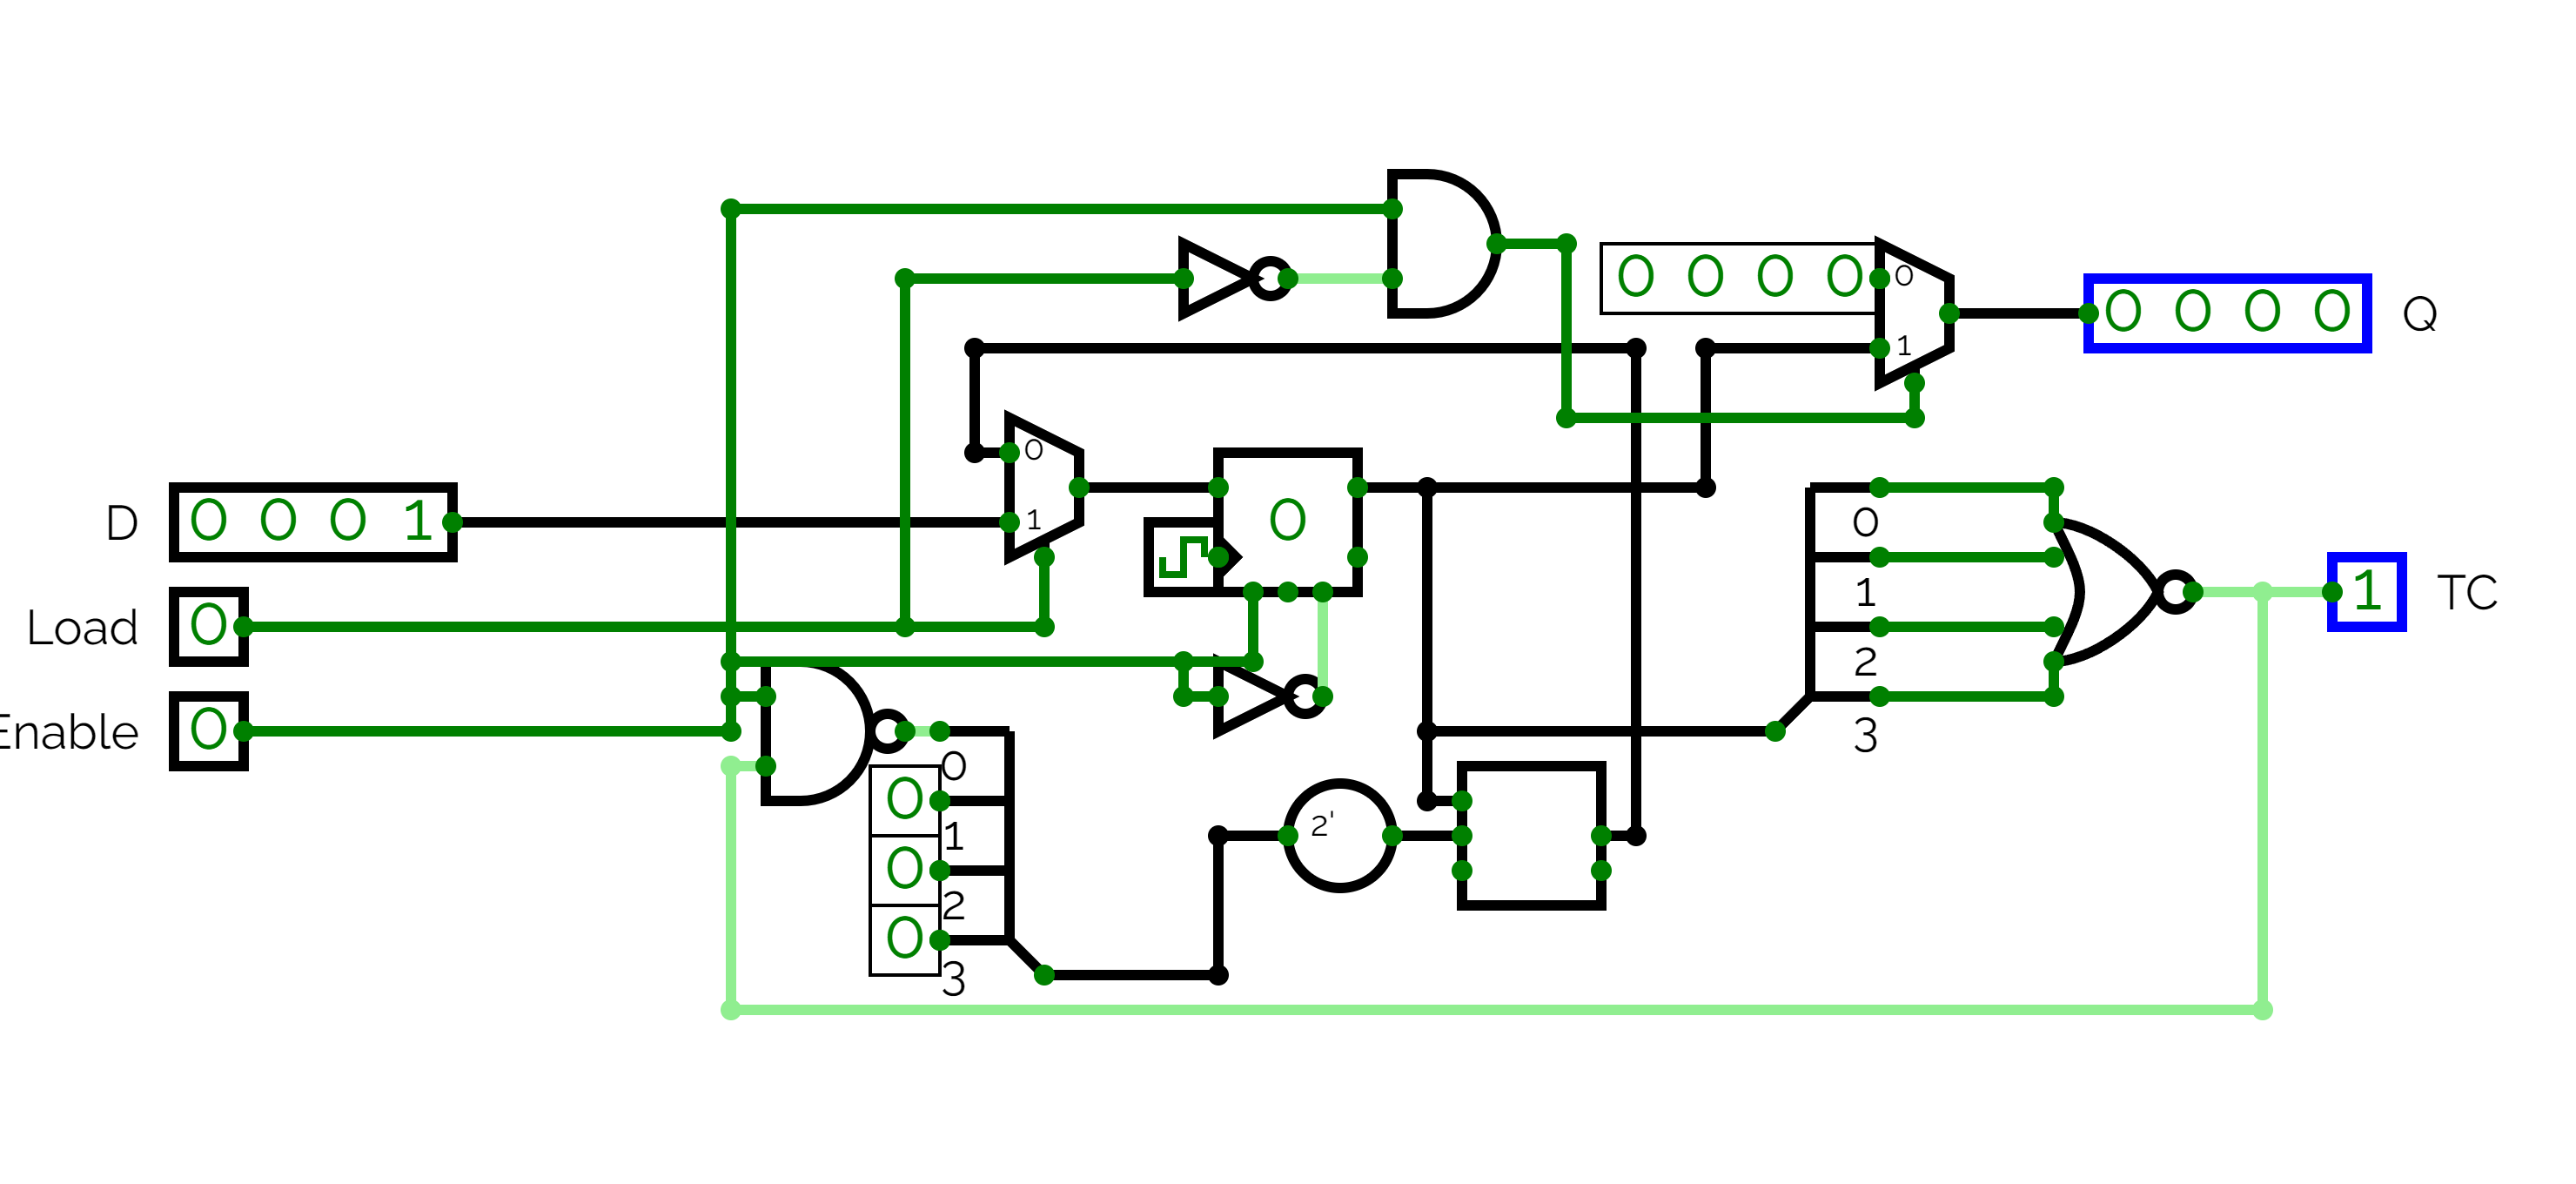
\includegraphics[width=0.8\textwidth]{Implementações/images/Counter Inside.png}
    \caption{Diagrama da lógica interna do Contador}\label{fig:Counter}
\end{figure}

Como podemos observar na figura acima, internamente, o contador contém um registo principal onde armazena o valor acumulado dos decrementos. Este registo é atualizado a cada ciclo de clock, decrementando o valor armazenado até atingir zero. Esta lógica é essencial para facilitar a integração com outros componentes do circuito. Considere agora a figura~\ref{fig:QuadradoCounter} que representa o diagrama do módulo Quadrado.

\begin{figure}[H]
    \centering
    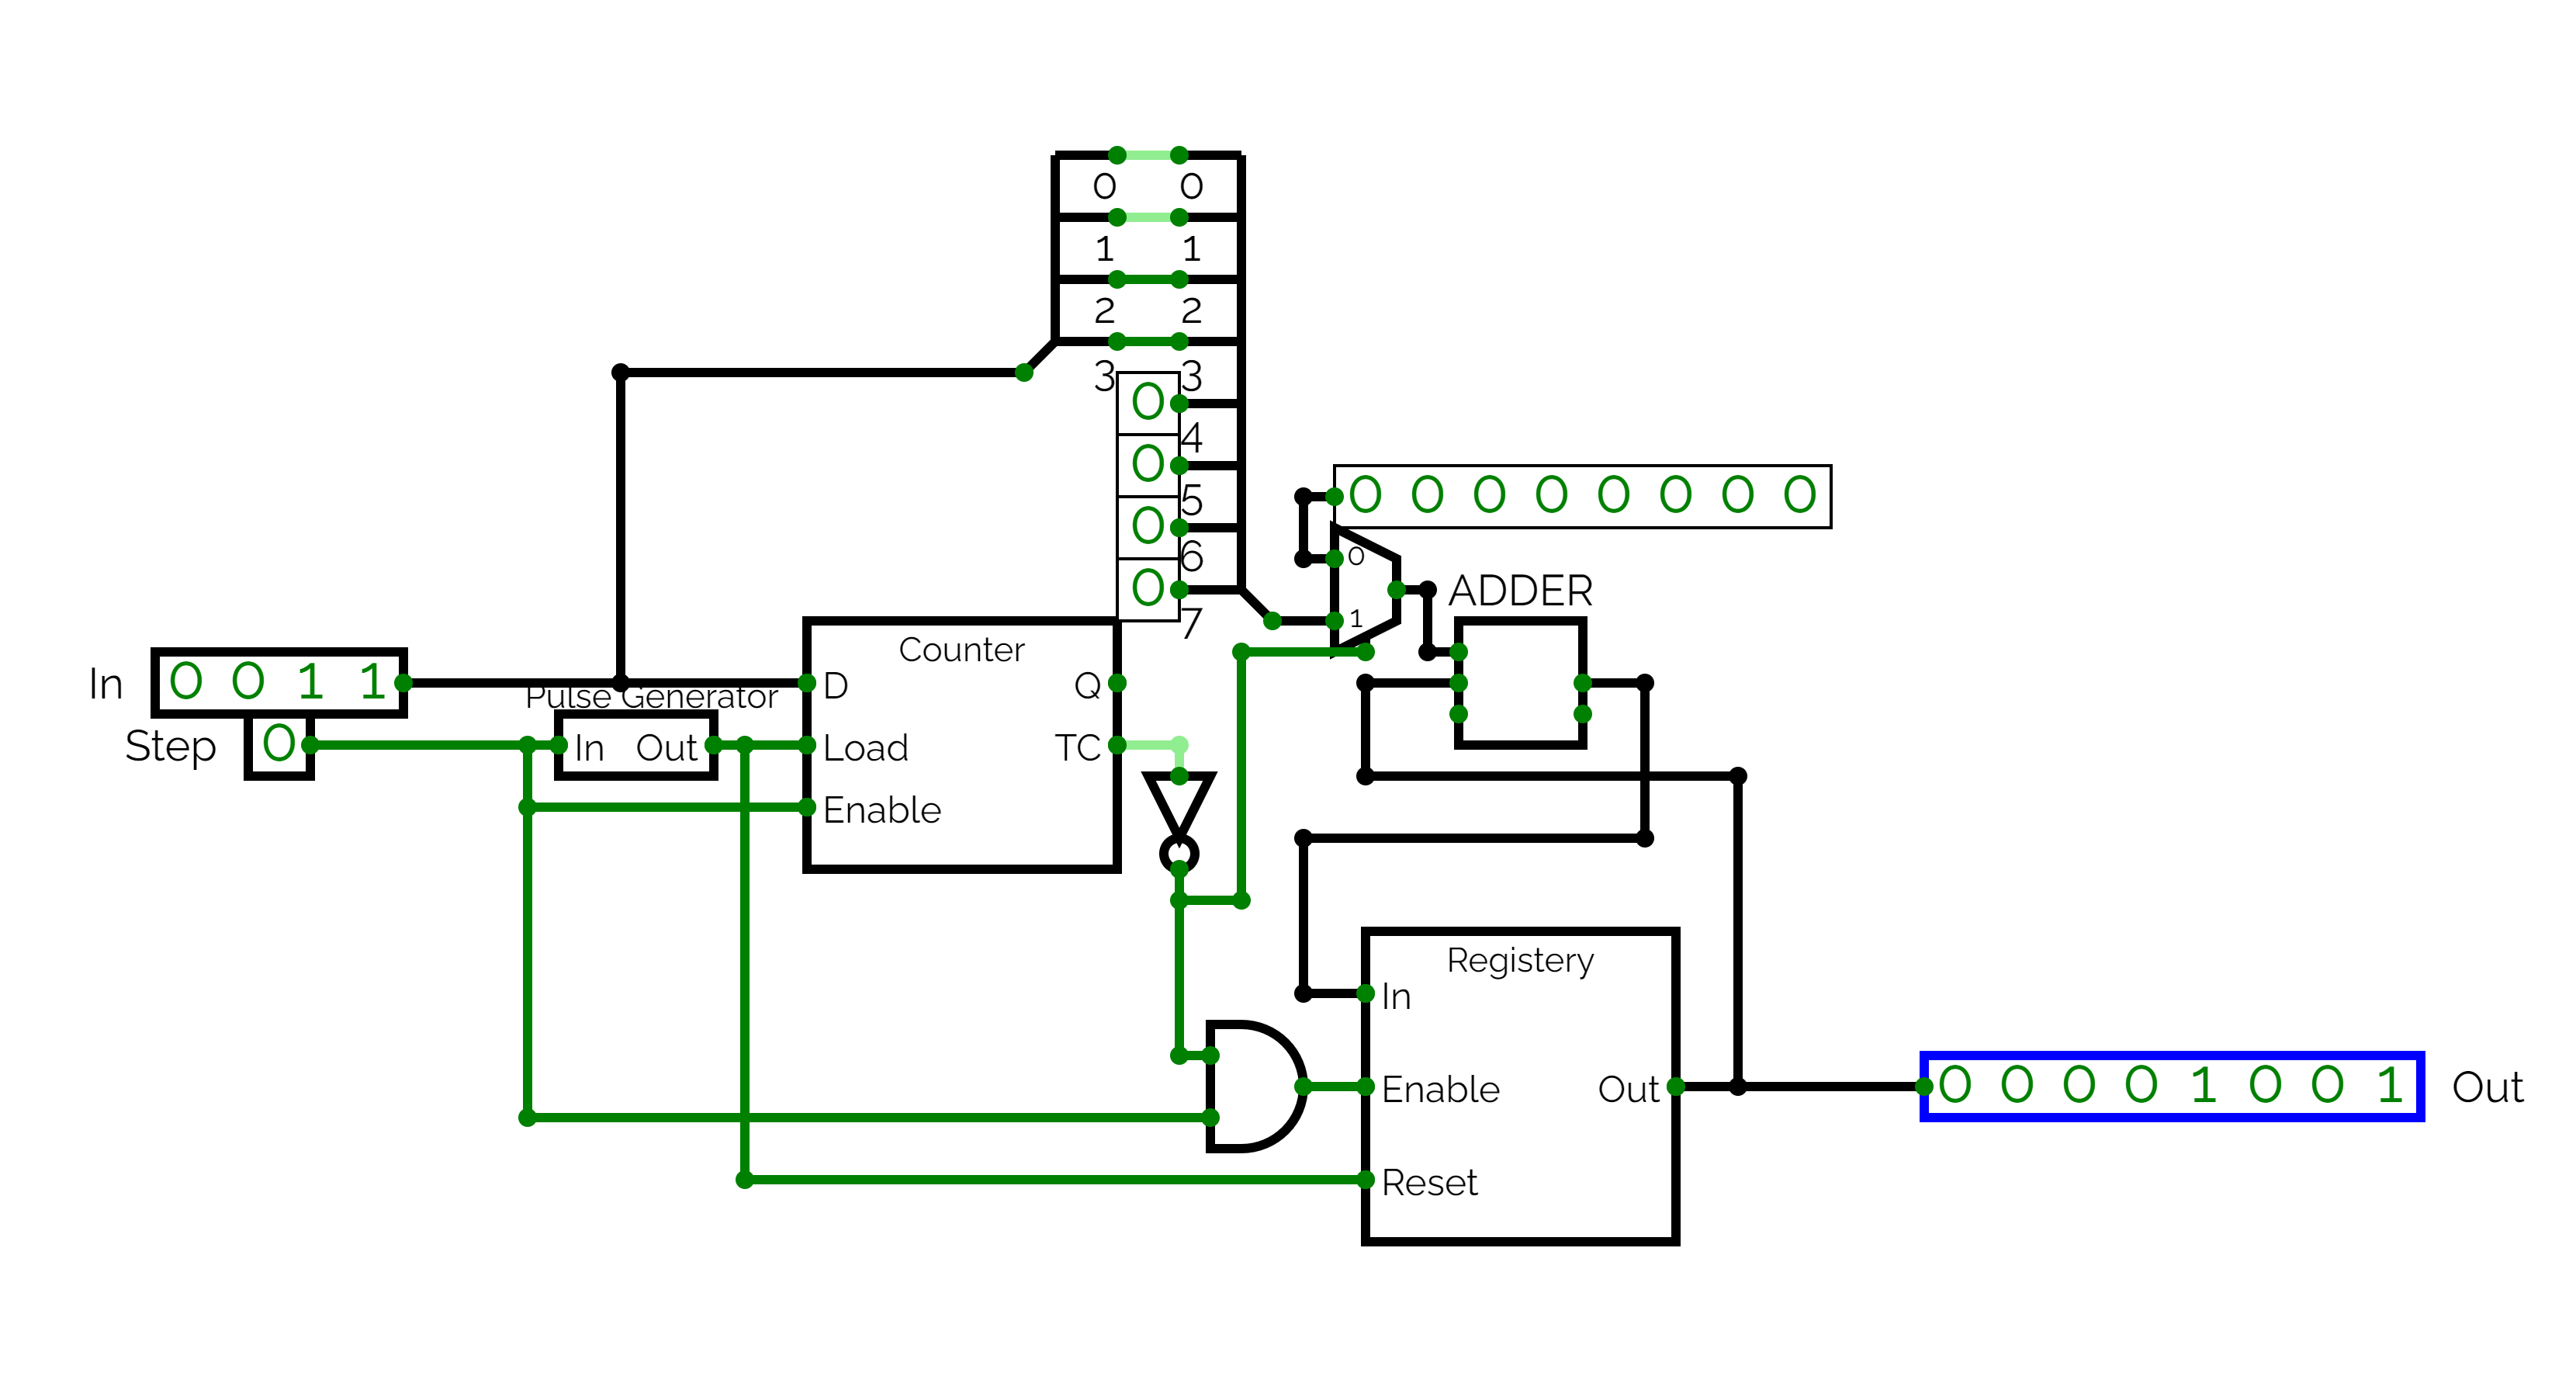
\includegraphics[width=0.8\textwidth]{Implementações/images/Counter.png}
    \caption{Lógica interna do Quadrado utilizando um contador}\label{fig:QuadradoCounter}
\end{figure}

O contador decrementa através do valor da entrada quando o step é premido. O Gerador de Pulso, que se situa entre a entrada Step e o contador, permite que o valor seja carregado num ciclo. Este comportamento é importante, pois impede o bloqueio das operações. Este sinal que sai do Gerador de Pulso, é também usado para reiniciar o registo que armazena a soma acumulada dos valores. Quando o contador chega ao zero, a saída TC (Terminal Count) é ativada, desativando o registo e comutando o \Gls{mux} a zero.

\begin{figure}[H]
    \centering
    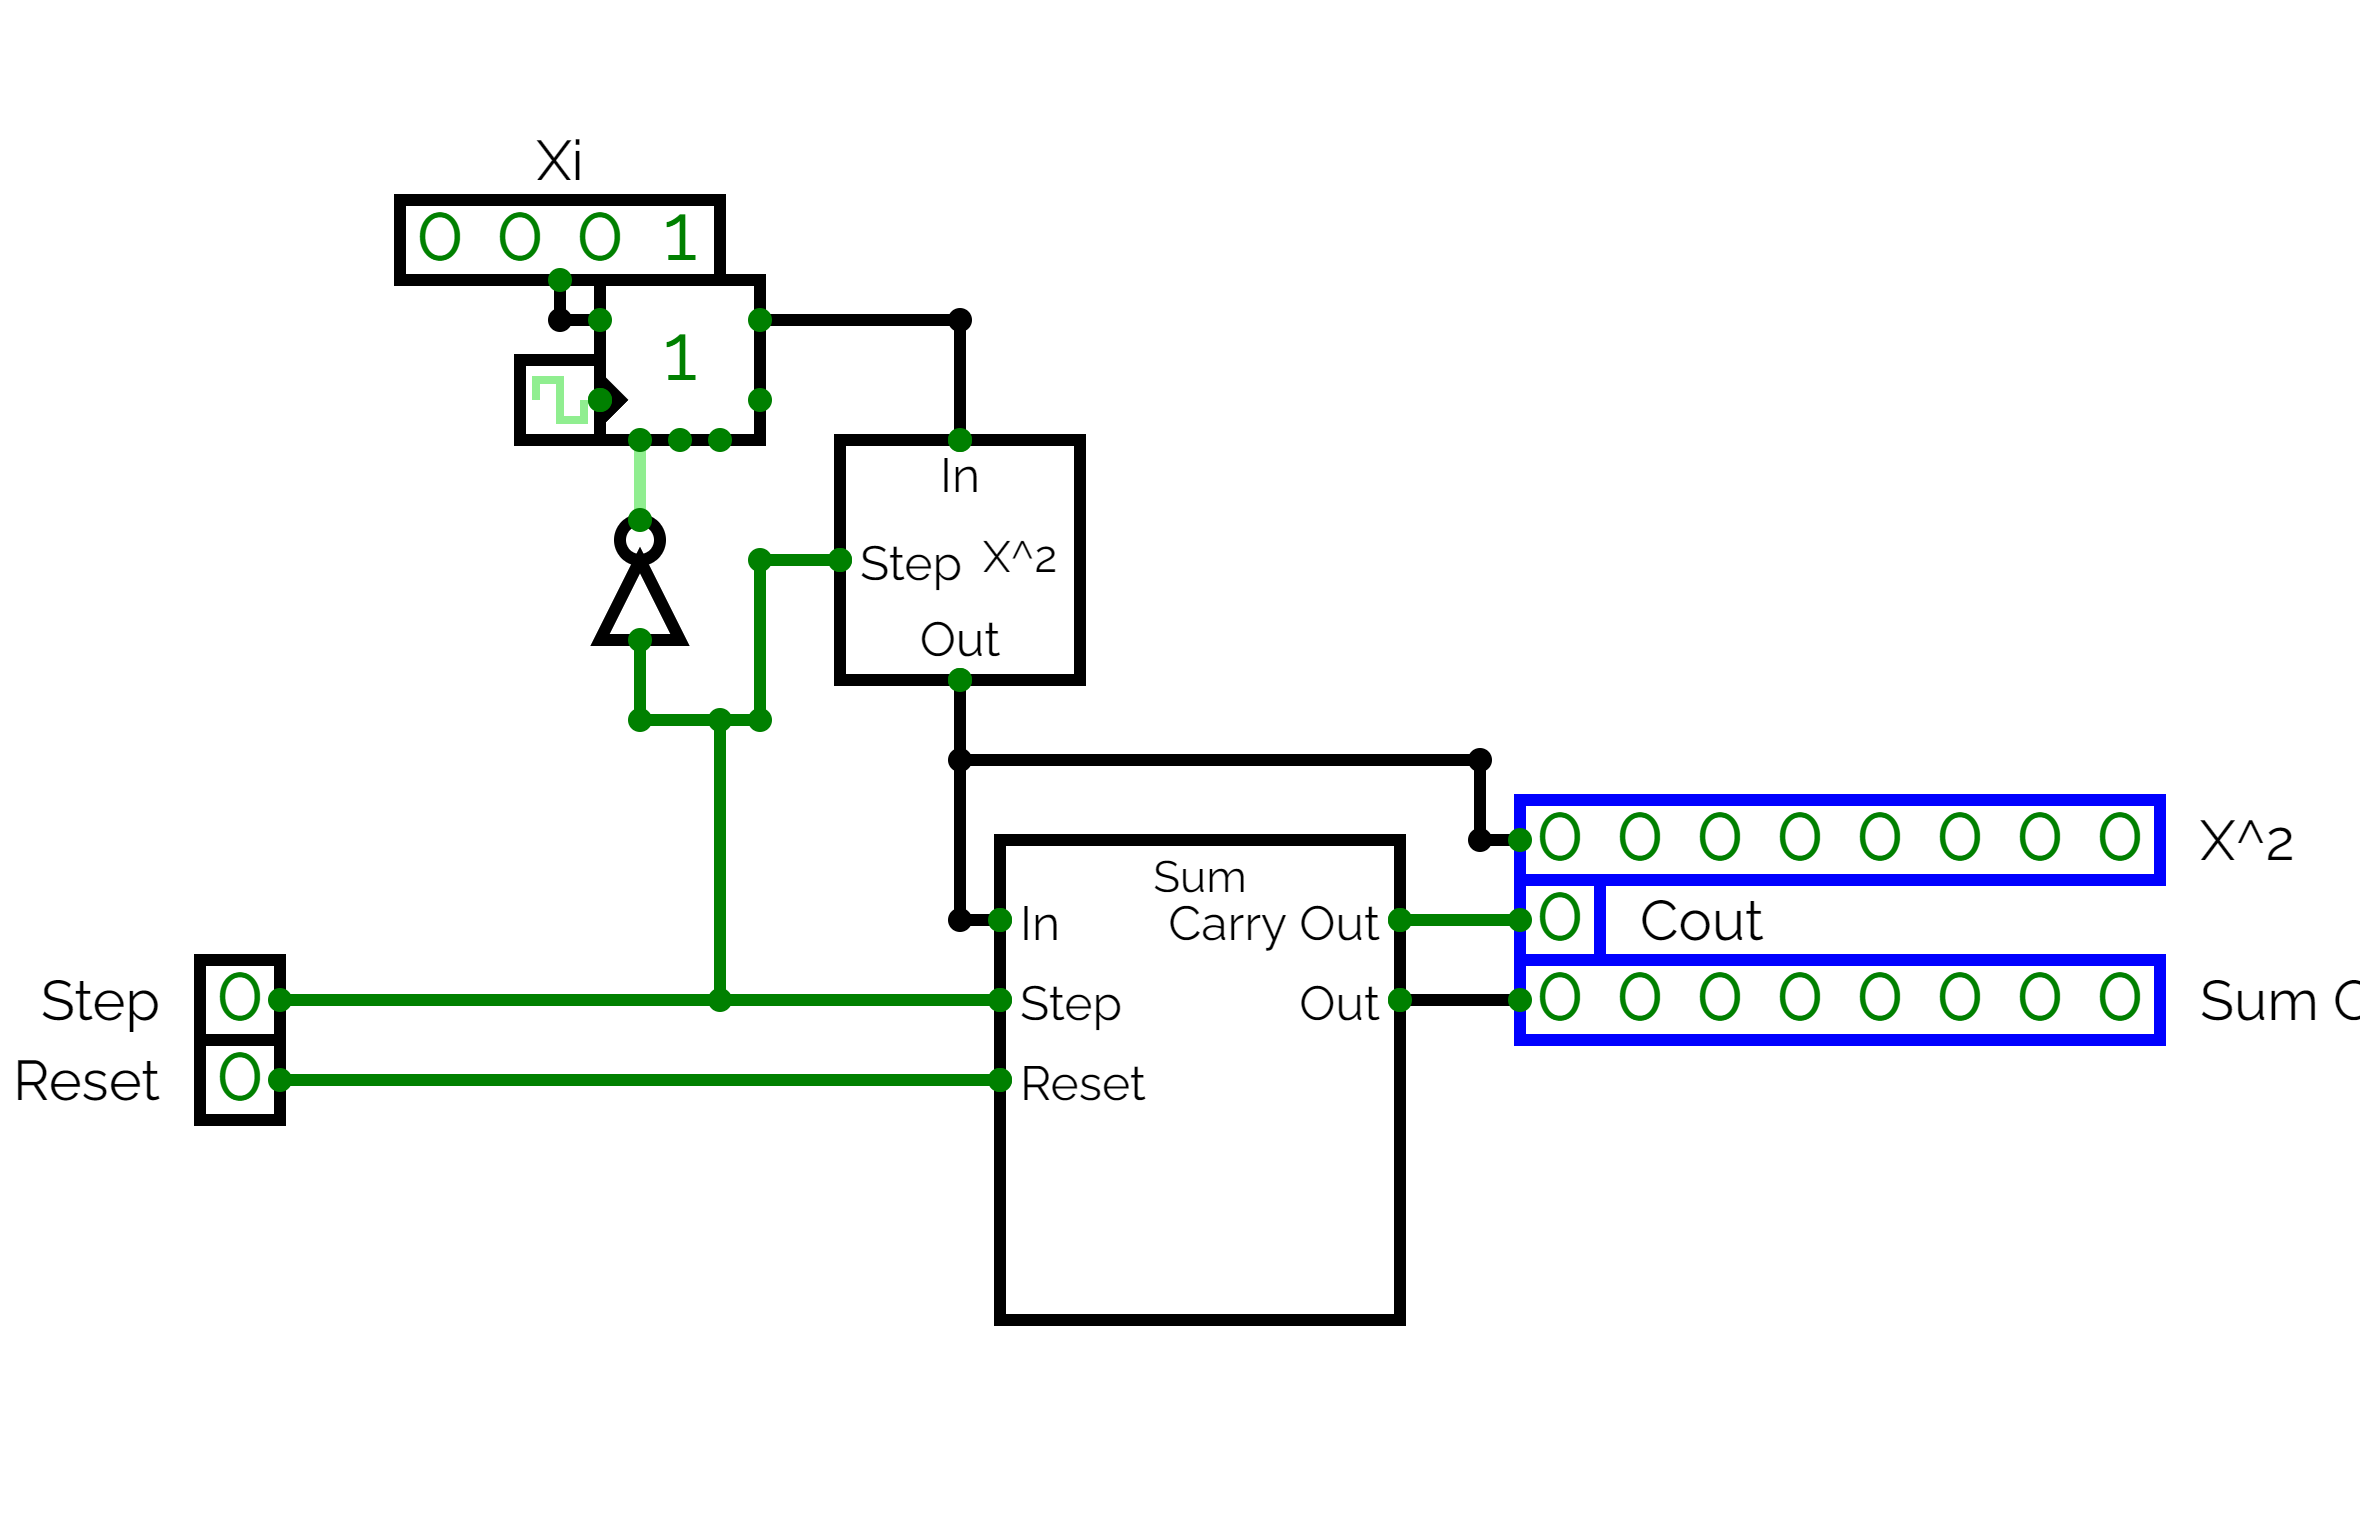
\includegraphics[width=0.8\textwidth]{Implementações/images/Counter DataPath.png}
    \caption{Lógica interna do Caminho de Dados utilizando o novo módulo Quadrado}\label{fig:QuadradoCounterDataPath}
\end{figure}

Esta abordagem introduz vários desafios relacionados com a temporização. Na prática, é consideravelmente mais complicada de implementar em relação às outras. Também notamos que, durante a simulação no CircuitVerse, esta implementação apresenta um desempenho inferior, especialmente para valores de entrada maiores, devido ao tempo adicional necessário para o contador percorrer todos os estados intermédios.

\subsection{Implementação Hardcoded}
Na implementação \gls{Hardcoded}, as operações e os comportamentos do sistema foram definidos diretamente em lógica fixa. Na prática, esta abordagem não é de todo prática e não apresenta nenhuma vantagem em relação às outras. Para além disso, carece de flexibilidade e adaptabilidade para alterações futuras no sistema. Como é possível observar na figura~\ref{fig:QuadradoHARD} abaixo, o nível de complexidade desta implementação aumenta exponencialmente.

\begin{figure}[H]
    \centering
    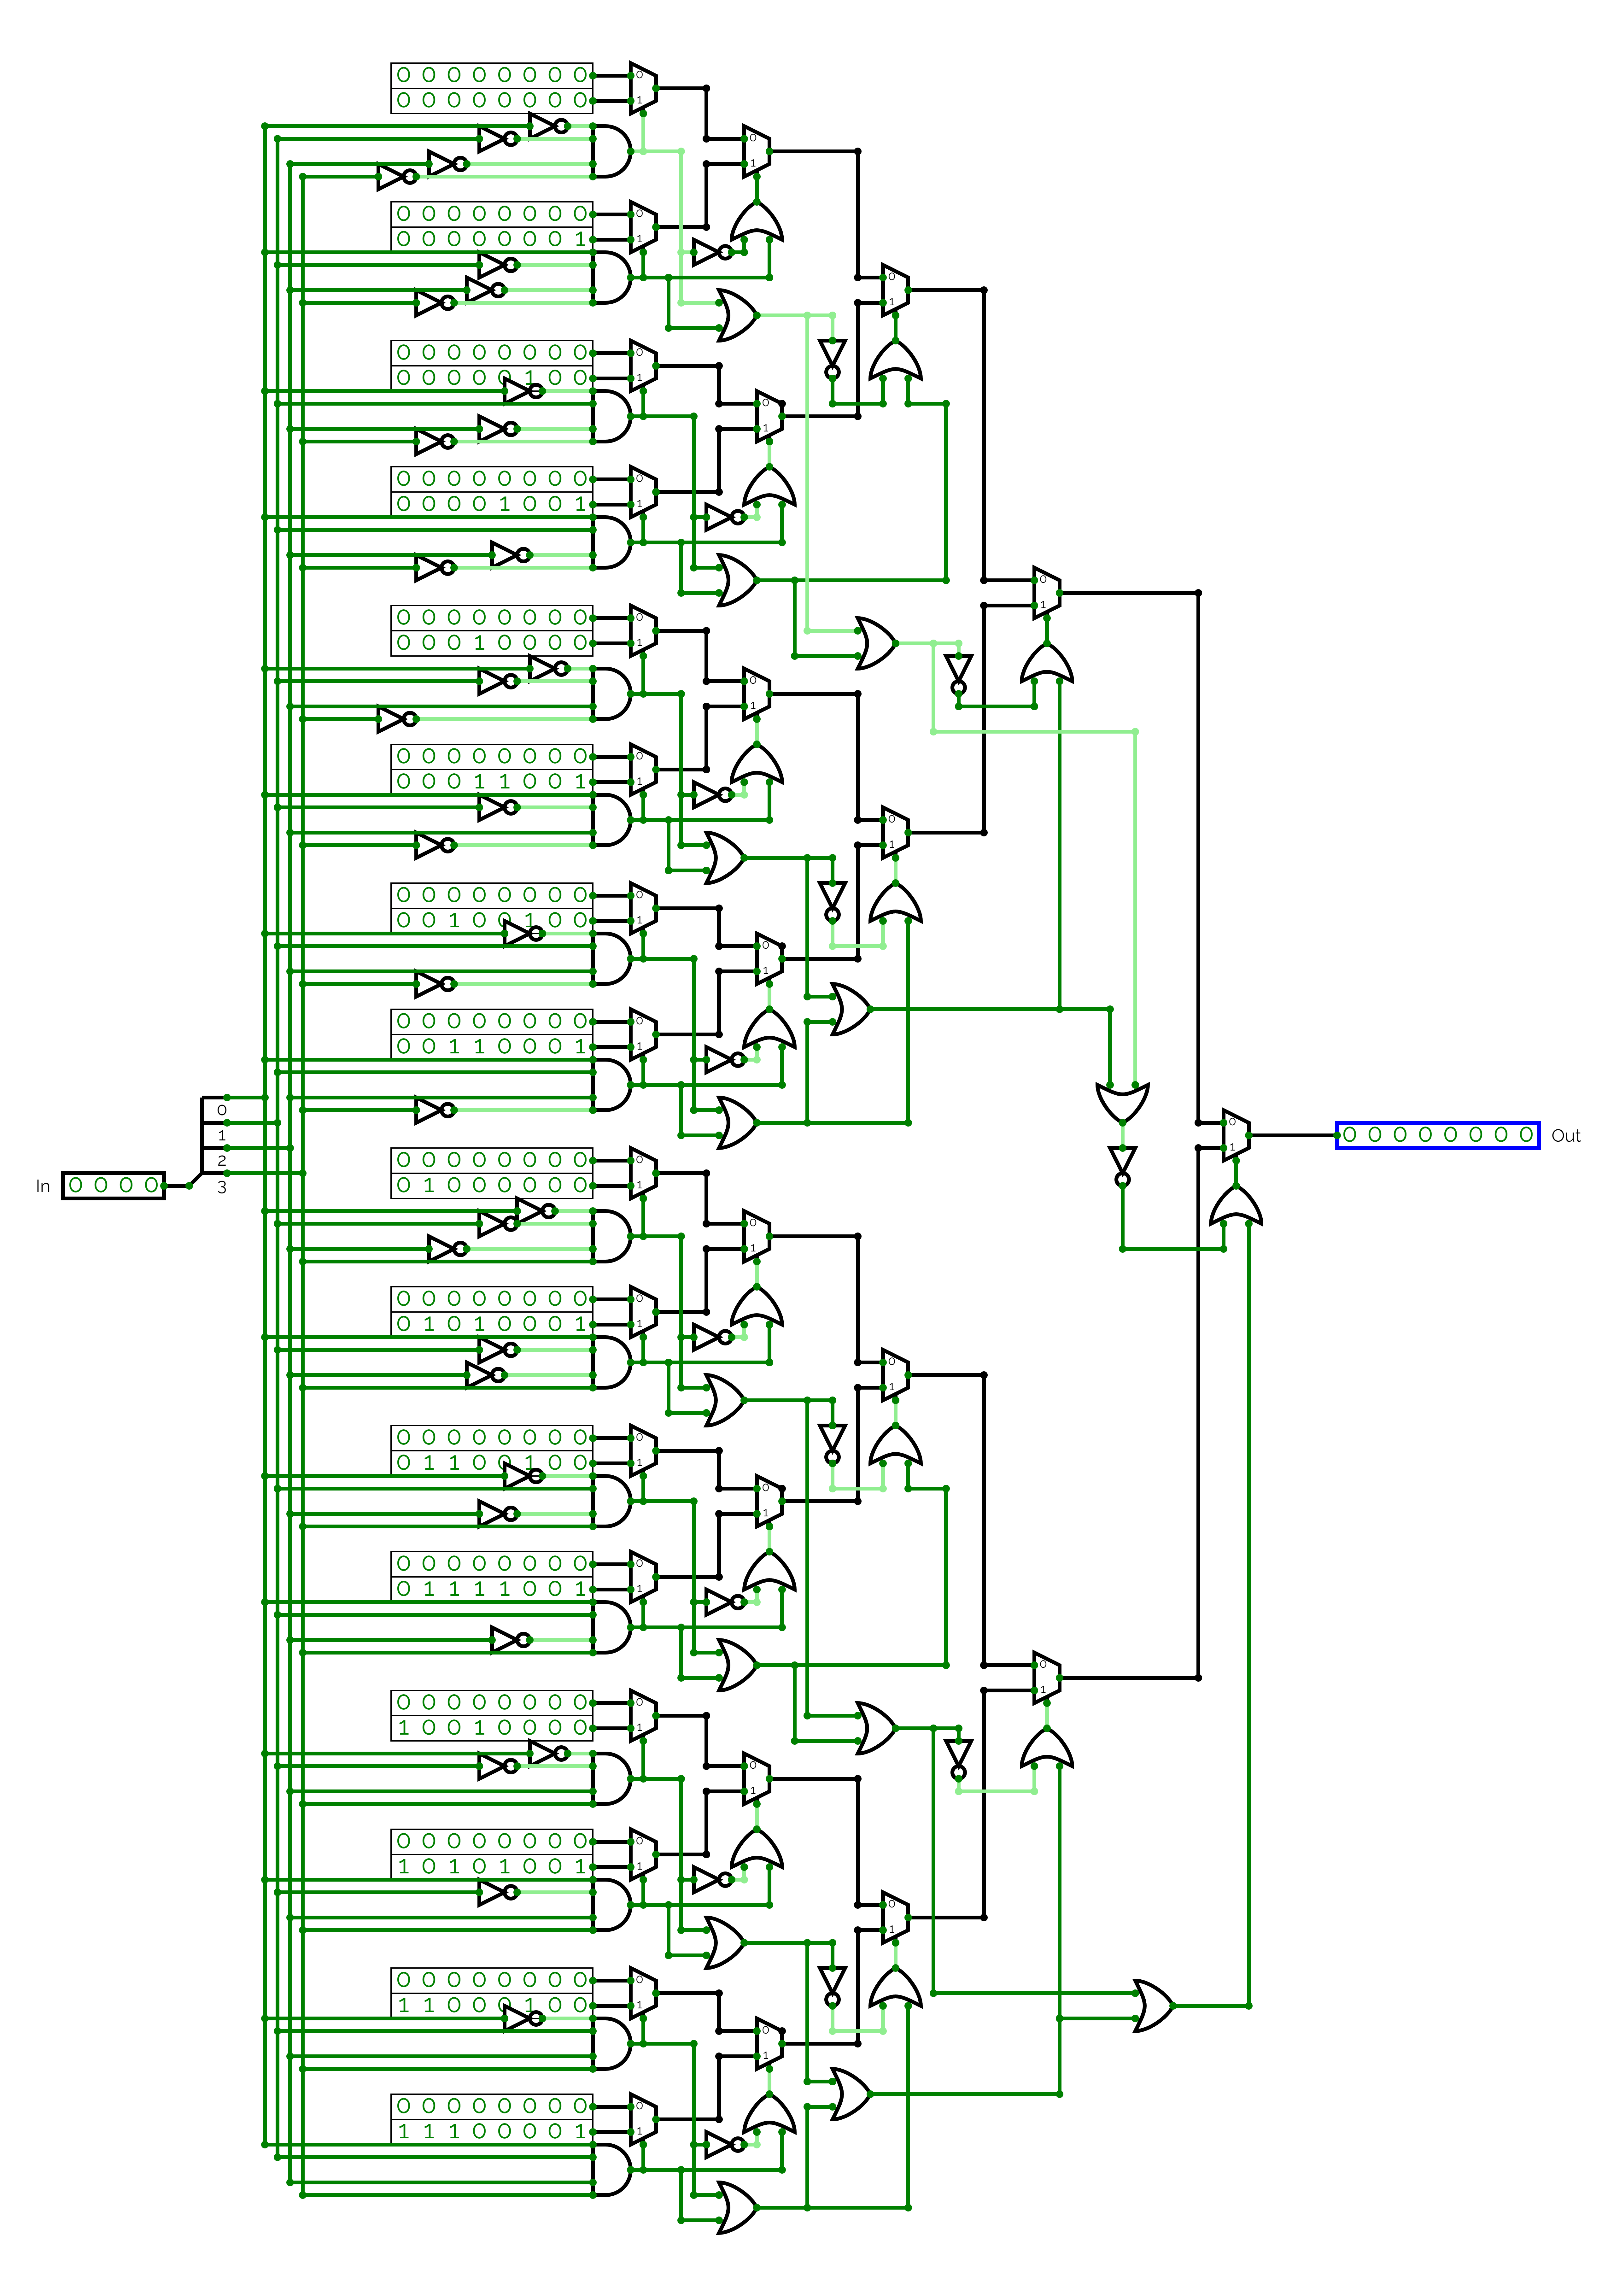
\includegraphics[width=0.7\textwidth]{Implementações/images/Hard.png}
    \caption{Implementação do módulo Quadrado Hardcoded}\label{fig:QuadradoHARD}
\end{figure}

\subsection{Comparação entre Implementações}

Neste subcapítulo, comparamos as diferentes abordagens analisadas, incluindo a implementação original baseada em \glspl{lsl}. A tabela~\ref{tab:ComparacaoImplementacoes} apresenta as principais vantagens e desvantagens de cada solução, permitindo uma avaliação mais detalhada sobre as características de cada uma.

\begin{table}[H]
    \centering
    \resizebox{\textwidth}{!}{%
    \begin{tabular}{|c|c|c|c|c|}
        \hline
        \rowcolor[HTML]{C0C0C0}
        \textbf{Critérios}                    & \textbf{Logic Shift Left} & \textbf{ROM} & \textbf{Contador} & \textbf{Hardcoded} \\
        \hline
        Fácil implementação                   & \checkmark                & \checkmark   & \xmark            & \checkmark         \\ \hline
        Bom desempenho para entradas médias   & \checkmark                & \checkmark   & \xmark            & \xmark             \\ \hline
        Eficiência para entradas altas        & \xmark                    & \checkmark   & \xmark            & \xmark             \\ \hline
        Flexibilidade para alterações futuras & \checkmark                & \xmark       & \checkmark        & \xmark             \\ \hline
        Simplicidade de design                & \checkmark                & \checkmark   & \checkmark        & \xmark             \\ \hline
        Dependente de ciclos de clock         & \xmark                    & \xmark       & \checkmark        & \xmark             \\ \hline
        Escalabilidade                        & \checkmark                & \xmark       & \checkmark        & \xmark             \\ \hline
    \end{tabular}%
}


    \caption{Comparação de Vantagens e Desvantagens das Diferentes Implementações.}
    \label{tab:ComparacaoImplementacoes}
\end{table}


A tabela acima fornece uma visão clara das características de cada abordagem, destacando os aspetos mais relevantes de cada solução. Dependendo das necessidades e restrições específicas, cada implementação pode ser mais ou menos adequada. Por exemplo, a solução original com \glspl{lsl} é uma escolha equilibrada, enquanto a abordagem com \gls{rom} pode ser ideal para sistemas que requerem rapidez e previsibilidade, mas com entradas limitadas.
